\documentclass[]{article}
\usepackage{lmodern}
\usepackage{amssymb,amsmath}
\usepackage{ifxetex,ifluatex}
\usepackage{fixltx2e} % provides \textsubscript
\ifnum 0\ifxetex 1\fi\ifluatex 1\fi=0 % if pdftex
  \usepackage[T1]{fontenc}
  \usepackage[utf8]{inputenc}
\else % if luatex or xelatex
  \ifxetex
    \usepackage{mathspec}
  \else
    \usepackage{fontspec}
  \fi
  \defaultfontfeatures{Ligatures=TeX,Scale=MatchLowercase}
\fi
% use upquote if available, for straight quotes in verbatim environments
\IfFileExists{upquote.sty}{\usepackage{upquote}}{}
% use microtype if available
\IfFileExists{microtype.sty}{%
\usepackage{microtype}
\UseMicrotypeSet[protrusion]{basicmath} % disable protrusion for tt fonts
}{}
\usepackage[margin=1in]{geometry}
\usepackage{hyperref}
\hypersetup{unicode=true,
            pdftitle={Presentation of Ancestral Reconstruction Results},
            pdfauthor={J.P. Meagher},
            pdfborder={0 0 0},
            breaklinks=true}
\urlstyle{same}  % don't use monospace font for urls
\usepackage{graphicx,grffile}
\makeatletter
\def\maxwidth{\ifdim\Gin@nat@width>\linewidth\linewidth\else\Gin@nat@width\fi}
\def\maxheight{\ifdim\Gin@nat@height>\textheight\textheight\else\Gin@nat@height\fi}
\makeatother
% Scale images if necessary, so that they will not overflow the page
% margins by default, and it is still possible to overwrite the defaults
% using explicit options in \includegraphics[width, height, ...]{}
\setkeys{Gin}{width=\maxwidth,height=\maxheight,keepaspectratio}
\IfFileExists{parskip.sty}{%
\usepackage{parskip}
}{% else
\setlength{\parindent}{0pt}
\setlength{\parskip}{6pt plus 2pt minus 1pt}
}
\setlength{\emergencystretch}{3em}  % prevent overfull lines
\providecommand{\tightlist}{%
  \setlength{\itemsep}{0pt}\setlength{\parskip}{0pt}}
\setcounter{secnumdepth}{0}
% Redefines (sub)paragraphs to behave more like sections
\ifx\paragraph\undefined\else
\let\oldparagraph\paragraph
\renewcommand{\paragraph}[1]{\oldparagraph{#1}\mbox{}}
\fi
\ifx\subparagraph\undefined\else
\let\oldsubparagraph\subparagraph
\renewcommand{\subparagraph}[1]{\oldsubparagraph{#1}\mbox{}}
\fi

%%% Use protect on footnotes to avoid problems with footnotes in titles
\let\rmarkdownfootnote\footnote%
\def\footnote{\protect\rmarkdownfootnote}

%%% Change title format to be more compact
\usepackage{titling}

% Create subtitle command for use in maketitle
\newcommand{\subtitle}[1]{
  \posttitle{
    \begin{center}\large#1\end{center}
    }
}

\setlength{\droptitle}{-2em}
  \title{Presentation of Ancestral Reconstruction Results}
  \pretitle{\vspace{\droptitle}\centering\huge}
  \posttitle{\par}
  \author{J.P. Meagher}
  \preauthor{\centering\large\emph}
  \postauthor{\par}
  \predate{\centering\large\emph}
  \postdate{\par}
  \date{8 January 2018}

\usepackage{tikz}
\usepackage{float}

\begin{document}
\maketitle

\section{Introduction}\label{introduction}

We are given a dataset of \(N\) bat echolocation call recordings denoted
\(\{y_n\}_{n = 1}^N\). This recording is then processed to produce a set
of smooth surfaces over a regular grid denoted
\(\{\tilde{S}_n\}_{n=1}^{N}\). This surface is produced by smoothing the
call spectrogram and mapping it to a regular grid over relevant
frequencies and an absolute time scale Pigoli et al. (2015).

\begin{figure}
\centering
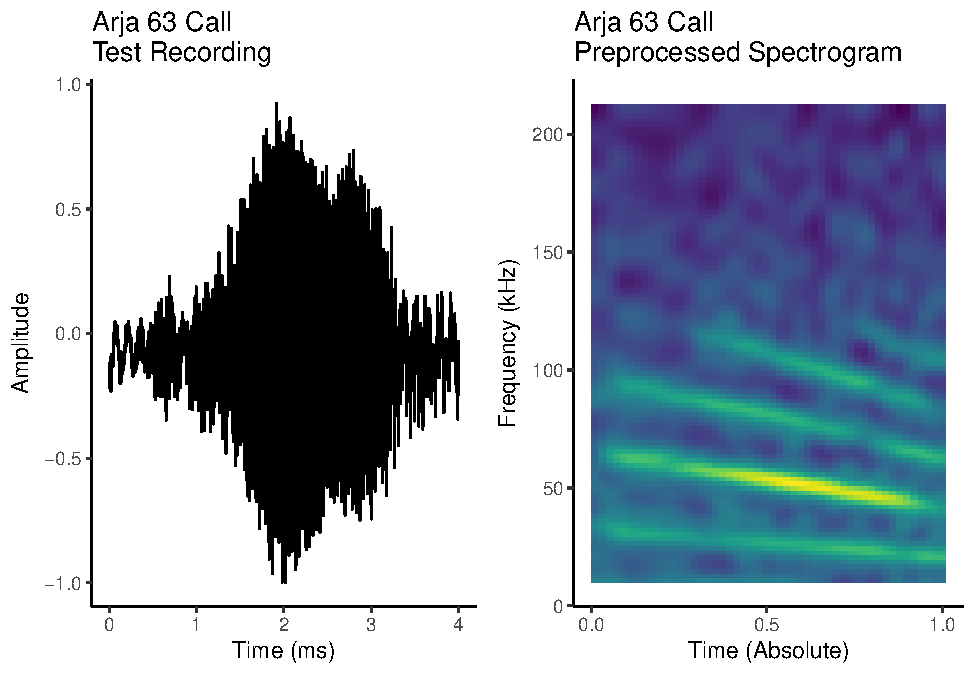
\includegraphics{for_mark_files/figure-latex/recording figure-1.pdf}
\caption{A randomly selected bat call from the species Arja alongside
it's corresponding smoothed surface representation. The smooth surface
is obtained by taking the call spectrogram and treating it as a
functional data object. The spectrogram is first smoothed by a robust
2-D spline smoother, then mapped to an absolute time scale and
registered in time by a pairwise surface synchronisation, and finally
restricted to the 9 - 212 kHz frequency spectrum.}
\end{figure}

Along with this dataset we are given a phylogeny defining the
evolutionary relationships between the species of bat.

\begin{figure}
\centering
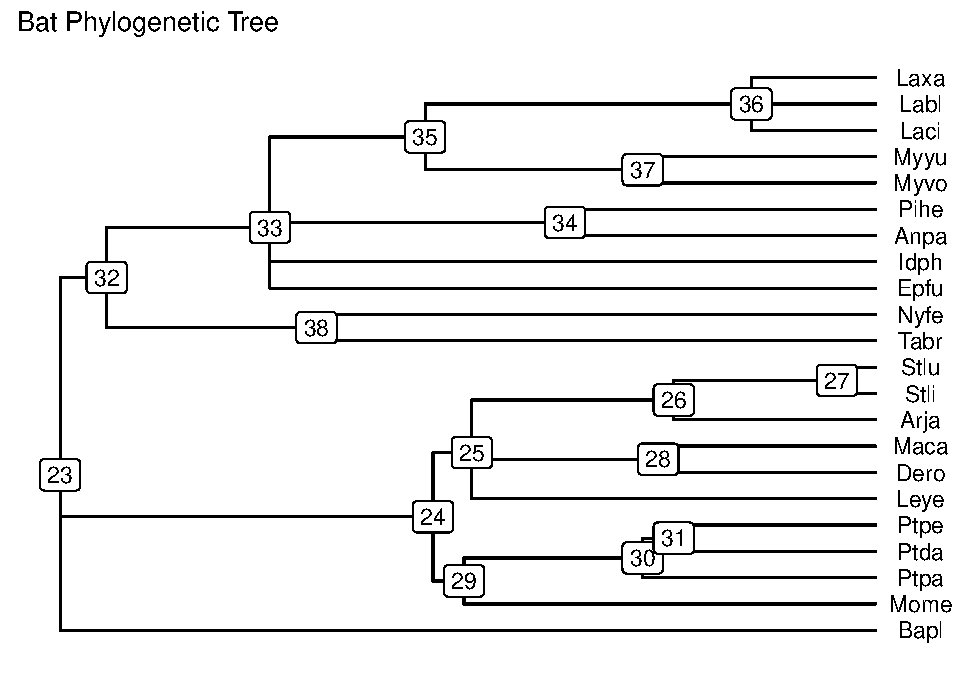
\includegraphics{for_mark_files/figure-latex/phylogeny figure-1.pdf}
\caption{Tree of assumed evolutionary relationships between Bat Species.
This phylogeny was transcribed from a recent bat super tree and shoud
represent a `best guess' for the evolutionary relationships between bat
species based on the fossil record alongside morphological and molecular
studies of evolutionary relationships.}
\end{figure}

A model has been developed to produce ancestral reconstructions for the
smoothed spectrogram surfaces representing the echolocation calls of
extinct bats and an audio file approximating the call that would
correspond to such a spectrogram surface can also be produced.

\begin{figure}
\centering
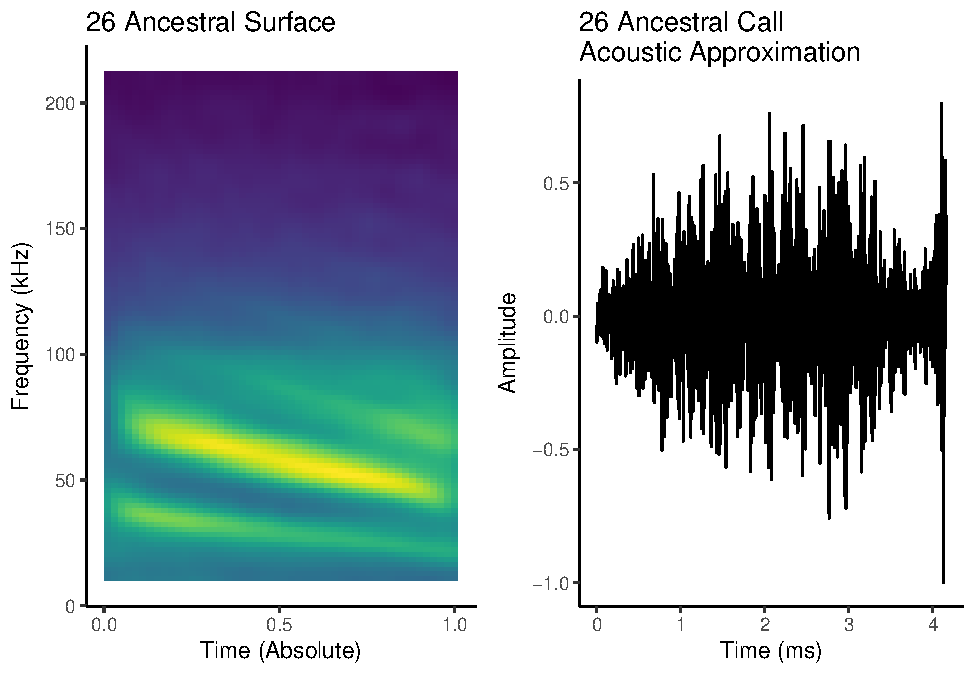
\includegraphics{for_mark_files/figure-latex/ancestral audio-1.pdf}
\caption{Ancestral spectrogram and acoustic approximation for the common
ancestor of Arja, Stli, Stlu. The reconstruction is given by the MAP
estimates for the weight of each evolutionary feature at the node. In
this case, evolutionary features were identified by a PCA of the
smoothed spectrogram surfaces. The acoustic reconstruction was performed
assuming a call duration of approximately 4 ms}
\end{figure}

Thus, for the dataset of Mexican Bat echolocation calls and the given
Phylogeny, Ancestral Reconstruction has been performed.

\section{The Current Model}\label{the-current-model}

An illustration of the current iteration of a model for the evolution of
bat echolocation calls is presented in Figure 4.

\tikzstyle{rv} = [circle, draw] 
\tikzstyle{plate} = [node distance = 1.25cm]

\begin{figure}
\centering
\begin{tikzpicture}[node distance = 2cm]
\node[rv, fill = gray!50, label = above left:$y_n$] (y) {};
\node[rv, fill = gray!50, label = above left:$S_n$, right of = y] (S) {}
edge[<-]  (y);

\node[rv, fill = gray!50, right of=S, label = above left:$w_{nq}$] (w) {}
edge[<-] (S);

\node[plate, above right of = w] (ntop) {};
\node[plate, below left of = y, label = 5:$N$] (nbot) {};
\draw[rounded corners] (ntop) rectangle (nbot) ;


\node[right of = w, label = above left:$\hat{w}_q$, rv] (hatw) {};
\node[above of = hatw, label = above left:$\theta_q$] (theta) {\textbullet}
edge [->] (hatw)
edge [<-] (w);
\node[right of = hatw, label = above right:$\mathcal{P}$] (P) {\textbullet}
edge [->] (hatw)
edge [->] (theta);
\node[below of = w, label = above right:$\phi_q$] (phi) {\textbullet}
edge [<-] (S)
edge [->] (w);

\node[plate, above right of = theta] (qtop) {};
\node[plate, below left of = phi, label = 5:$Q$, ] (qbot) {};
\draw[rounded corners] (qtop) rectangle (qbot);

\node[rv, below of=P, label = below left:$\hat{S}$] (hatS) {}
edge[<-] (hatw)
edge[<-] (phi);
\node[right of=hatS, label = below left:$\hat{y}$] (haty) {\textbullet}
edge[<-] (hatS);
\end{tikzpicture}
\caption{A Graphical model detailing the structure of the model for evolution used to produce reconstructions of ancestral bat echolocation calls. Let \(y_n\) be a random variable representing an echolocation call recording. \(S_n\) is the random variable representing the smoothed spectrogram surface given by \(y_n\). The Mexican bat call dataset provides \(N = 1816\) observations of these random variables. The process of transforming a call recording into a spectrogram surface was covered in my 9 month report. The model assumes that each \(S_n\) can be modelled by \(Q\) independent deterministic 'evolutionary features' denoted \(\phi_q\). In this case \(\phi_q\) is inferred by a Principal Components Analysis of \(\{S_n\}_{n = 1}^N\). The weight of each evolutionary feature in \(S_n\) is itself a random variable, where \(w_{nq}\) denotes the weight of \(\phi_q\) in \(S_n\). \(w_{nq}\) is assumed to behave as an Ornstein-Uhlenbeck Gaussian process for which the input space is the phylogeny \(\mathcal{P}\). Each Gaussian process is defined by the deterministic hyperparameters \(\theta_q = [\gamma_q, \ell_q, \sigma_q]^\mathsf{T}\) which are inferred from the data by Type II maximum likelihood estimation over the observed weights. The phylogeny \(\mathcal{P}\) is also assumed to be deterministic in this model and is shown in Figure 2. Ancestral reconstruction is performed by making a prediction for the feature weights, denoted \(\hat{w}\), at some point on \(\mathcal{P}\). Applying these weights to the evolutionary features produces the ancestral call surface which in turn provides an estimate for the ancestral call.}
\end{figure}

\section{A Joint model for spectrogram
surfaces}\label{a-joint-model-for-spectrogram-surfaces}

\begin{figure}
\centering
\begin{tikzpicture}[node distance = 2cm]
\node[rv, fill = gray!50, label = above left:$y_n$] (y) {};
\node[rv, fill = gray!50, label = above left:$S_n$, right of = y] (S) {}
edge[->]  (y);

\node[rv, right of=S, label = above right:$w_{q}$] (w) {}
edge[->] (S);

\node[plate, above right of = S] (ntop) {};
\node[plate, below left of = y, label = 5:$N$] (nbot) {};
\draw[rounded corners] (ntop) rectangle (nbot) ;

\node[above of = w, label = above right:$\theta_q$] (theta) {\textbullet}
edge [->] (w);
\node[right of = w, label = above right:$\mathcal{P}$] (P) {\textbullet}
edge [->] (w);
\node[below of = w, label = above right:$\phi_q$] (phi) {\textbullet}
edge [->] (S);

\node[plate, above right of = theta] (qtop) {};
\node[plate, below left of = phi, label = 5:$Q$, ] (qbot) {};
\draw[rounded corners] (qtop) rectangle (qbot);

\node[rv, below of=S, label = below left:$\hat{S}$] (hatS) {}
edge[<-] (w)
edge[<-] (phi);
\node[below of=y, label = below left:$\hat{y}$] (haty) {\textbullet}
edge[<-] (hatS);

\node[above of = S, label = above left:$\Sigma$] (phi) {\textbullet}
edge [->] (S);
\end{tikzpicture}
\caption{A proposed extension to the model for the evolution a bat echolocation calls presented in Figure 4. This model includes a noise process over the call surface, which would allow the calculation of the model evidence. This in turn would facilitate model selection for various sets of evolutionary features, phylogenies, and Ornstein-Uhlenbeck process hyperparameters.}
\end{figure}

\hypertarget{refs}{}
\hypertarget{ref-pigoli2015analysis}{}
Pigoli, Davide, Pantelis Z Hadjipantelis, John S Coleman, and John AD
Aston. 2015. ``The Analysis of Acoustic Phonetic Data: Exploring
Differences in the Spoken Romance Languages.'' \emph{arXiv Preprint
arXiv:1507.07587}.


\end{document}
